%Remaining Anonymous when using the Bitcoin Protocol
\section{Introduction}
% Computer Society journal papers do something a tad strange with the very first
% section heading (almost always called "Introduction"). They place it ABOVE the
% main text! IEEEtran.cls currently does not do this for you.  However, You can
% achieve this effect by making LaTeX jump through some hoops via something
% like:
%
%\ifCLASSOPTIONcompsoc \noindent\raisebox{2\baselineskip}[0pt][0pt]%
%{\parbox{\columnwidth}{\section{Introduction}\label{sec:introduction}%
%\global\everypar=\everypar}}% \vspace{-1\baselineskip}\vspace{-\parskip}\par
%\else \section{Introduction}\label{sec:introduction}\par \fi
%
% Admittedly, this is a hack and may well be fragile, but seems to do the trick
% for me. Note the need to keep any \label that may be used right after \section
% in the above as the hack puts \section within a raised box.



% The very first letter is a 2 line initial drop letter followed by the rest of
% the first word in caps (small caps for compsoc).
% 
% form to use if the first word consists of a single letter:
% \IEEEPARstart{A}{demo} file is ....
% 
% form to use if you need the single drop letter followed by normal text
% (unknown if ever used by IEEE): \IEEEPARstart{A}{}demo file is ....
% 
% Some journals put the first two words in caps: \IEEEPARstart{T}{his demo} file
% is ....
% 
% Here we have the typical use of a "T" for an initial drop letter and "HIS" in
% caps to complete the first word.
%\IEEEPARstart{T}{his}

\IEEEPARstart{A}{t 6:15 pm} on the 3rd of January 2009, Satoshi Nakamoto (likely a pseudonym) created and announced a block of data known as the `Genesis Block' of the Bitcoin block chain~\cite{satoshi}. With this block, the first 50 units of the decentralized peer to peer currency, Bitcoin, were created\footnote{Strictly this isn't true, as due to a bug in the bitcoin client the first 50 bitcoins created cannot actually be spent.}. Since then, over ten million bitcoins have been generated.

The \textcite{euro-currency-schemes} (ECB) describes three different virtual currency schemes: closed currency schemes, unidirectional and bidirectional flow currency schemes.  Closed currency schemes involve currencies that cannot be converted to or from fiat currency\footnote{Fiat currency is a currency with a value given by government regulation such as the Great British Pound (GBP) or the United States Dollar (USD)}, an example of this would be `World of Warcraft gold'\footnote{\url{http://eu.battle.net/wow/en/shop/anti-gold/}} which cannot be bought using legal tender without violating the terms of service.  Unidirectional currency schemes include currencies like `Facebook Credits'\footnote{\url{https://www.facebook.com/credits/}} that can be purchased using legal tender but cannot be transfered to other users.  Finally, bidirectional currency schemes describe currency which can be converted to and from fiat currency, bitcoins are an example of this and are currently trading at \input{price}.

Bitcoin is distinct from other bidirectional digital currency schemes such as central banking and financial institutions or money transfer systems such as PayPal\cite{paypal} in that ``it is neither created nor administered by a single authority such as a central bank''\cite{why-interesting}, transactions are also irreversible are made pseudo-anonymously. The bitcoin protocol allows multiple different clients to connect, verify and disseminate transactions.  The reference bitcoin client, has received multiple releases\footnote{\url{http://bitcoin.org/en/version-history\#0.5.0}} and is now known as Bitcoin-Qt\cite{bitcoin-qt}. For the sake of brevity this paper will refer to Bitcoin-Qt Bitcoin client as the Bitcoin client.

\section{Related Work}
Research on the Bitcoin protocol has mostly centered around proposing improvements to the protocol, such as the \textcite{red-balloons} who sugggest a reward scheme for ensuring bitcoin peers re-broadcast transaction messages, or \textcite{bitter-to-better} that looks at a multitude of different proposals for improvement such as improving the scalibility of transaction history storage.  Other research such as that of \textcite{legal}, focus on the legal status of bitcoin as a currency.  This research paper focusses on the emergance of Bitcoin  within the context of both theoretical and implemented digital currency systems and a critical assessment of the anonymity of the Bitcoin protocol.

\section{Background}
The core of any currency is to allow users to participate in transactions that result in transfer of value between the participants.  Such a system requires an element of trust or protocols that remove the need for trust between the participants.  If a user, Alice, wishes to send some value to Bob, Bob will need to know that Alice has the funds to send that transaction and has not sent or allocated that money to anyone else (a double spend). This problem is easily solvable using a physical transferable goods where the expense to duplicate or create more of a resource can be ensured to be more than the value of the item: for example creating counterfeit paper currency or creating a commodity like gold.  Although the issue of trust is somewhat negated with physical goods, they also encounter a separate issue - moving that value over distance.  This can be an expensive exercise as it requires both the expense of physically moving the good - particularly an issue with heavy gold bars - as well as the cost of securing it during transportation. While paper currencies solve these problems somewhat, with a trade-off of making duplication easier, a digital currency aims to recreate the difficulty in duplication, while taking advantage of the ease of transfer that digital information brings.

Up until relatively recently, discussions in scientific literature surrounding currency systems have assumed the necessity of some type of trusted central authority or authorities as part of the operation of the protocol.  These authorities usually maintain a record of transactions performed as well as minting and controlling the currency.  However, the relative success of Bitcoin has shown that this assumption is not necessarily the case and has increased discussion into decentralised currency - moving it from a topic of intellectual curiosity to one with more practical implications.

\subsection{Central Banking Authorities}

Services  such as the UK ``Faster Payments  Service''~\cite{guardian-fps}, or the  ``Single Euro Payments Area''  (SEPA) payments initiative~\cite{SEPA}  operates as a transfer protocol or interchange, between trusted  entities such as banks and other financial institutions.  These transfer  protocol systems transfer  actual units of currency, in the case of SEPA, actual Euros.  This is  in contrast to payment processor systems and services such as PayPal\footnote{\url{https://www.paypal.com/uk/webapps/mpp/transfer-money-online}}, Dwolla\footnote{\url{https://www.dwolla.com/individuals}} and Liberty Reserve\footnote{\url{http://web.archive.org/web/20130430103158/http://www.libertyreserve.com/}} which utilise equivalent tokens rather than actual currency within it's transactions.  These equivalent tokens are only utilised within the PayPal system and are not trade-able outside of these transfers while maintaining a 1:1 conversion rate with actual currency. This equivilent credit is transferred between users by debiting one user and crediting the other which can later be exchanged for actual currency~\cite{paypal}.  PayPal itself transfers money around its organisation via SEPA thus, is not a transfer protocol but operates on top of it.

While there are legal distinctions between financial institutions' transfer systems and payment processors,  there is no significant technical distinction.  These systems are  effectively centralized, digital systems of exchange in which only the  central authority or authorities control the minting of the currency or  are able to create transactions.  An individual cannot create  transactions and must rely on the central authority to make the  transaction on their behalf.

These  fully centralized systems have a simple design and implementation and often provides useful features such as insurance and interest.  However,  there are some key issues that affect the users of the system -  both  merchants and customers - two of which are discussed  below.

The  first issue is that the central authority has a legal responsibility to  handle ``charge-backs'' or reverse transactions.   The  cost for this escrow service - in which the central authority acts as  an arbiter in  disputes - is placed on the customer as a transfer fee or  to the  merchant as a fine.  In cases of arbitration the participants within the transaction are wholly  subject to the central authorities decision and there have been several  high profile cases that have highlighted the way that arbitration can  be mishandled by a central authority ~\cite{violin}.   While arbitration can be useful, it results in the disenfranchising of  the users of the system because the users are not truly in control of  their own funds as they would be in the case of a physical currency.

The second major disadvantage of a centralized system is that it allows  for  a single point of failure resulting in a lack of reliability from   the  perspective of the user.  The central authority has complete  control over the status of the users' account - that authority can   freeze the funds of that account at their discretion according to their  own terms of service, this can include pressure from legal  authorities~\cite{mtgox-dwolla,vlad:mtgox-dwolla,wikileaks-paypal}.   Additionally, the central authority exists as an easier target for  legal  action, should that authority fail to freeze or track  `problematic'  accounts and this may result in a total shut down of  that  service~\cite{lr-shutdown,egold-shutdown,lr-idictment}. This  report assumes that being resilient  to attack from a third party, regardless of the good intentions of that  party, is an advantageous feature of a  currency.  It is not in the  scope of this report to discuss the legal or ethical repercussions of  such a system.

\subsection{Unique Token}
\textcite{netcash} discuss one solution, NetCash.  This protocol uses a unique token held by both the central authority and the owner of the coin. To create NetCash currency, the user and central authority agree on a unique token in exchange for some currency or resource. When that user wishes to transact value to another, they simply send the token to the other user.  A receiver can opt to trust the sender, thus remaining anonymous, or can trade-off anonymity for an assurance of validity from the central server.  To verify that the transaction is legitimate, receiving users send the token to the exchange, to be swapped for a new spendable token meaning the original token can no longer be spent. One issue with this protocol is the central authority cannot be independently verified, as such the central server may deny knowledge of a valid token, or allow multiple users to claim the same token and arbitrarily mint new tokens without a fee (either maliciously, due to being compromised or due to data loss).

\subsection{Blind-signed Chaumian e-Cash}
Proposed by \textcite{chaum}, the Chaum Token protocol, uses blind signatures. A user, Alice, creates a token $x$ and blinds it using function $c$.  A central authority will sign this blinded message using signing function $s$ in exchange for a fee, creating $s(c(x)$.  The authority then returns the blind signed message to Alice. Alice then removes the blind, leaving the signature $s(x)$ using $c^{-1}(s(c(x)))$.  These signed messages can now operate in a similar manner to tokens from the NetCash system: Alice can send $s(x)$ to Bob, who verifies the central authority's signature, and is now able to redeem this token with the central authority preventing Alice from sending the same token to another user.

The blinding protocol has the advantage that the central authority cannot discover the previous owner of a signed message when cashed by a payee because it is assumed that $c(x)$ cannot be derived from $s(x)$.  This protocol, however, maintains similar issues to NetCash: the central server may allow multiple users to claim the same token and arbitrarily mint new tokens without a fee (either maliciously, due to being compromised or due to data loss).

In both NetCash and Chaumian e-Cash the central server may accuse the original owner of the token of double spending the transaction.  Assuming Alice did not double spend the token, she now knows that the central server is dishonest, Bob on the other-hand cannot determine which of Alice or the central authority are being dishonest.

\subsection{B-Money digital signature chain}\label{digital-sig}
An alternative solution, B-Money proposed by~\textcite{b-money}, uses a chain of digital signatures where transaction messages are created using public key cryptography and the chain of digital signatures can be traced back to the original creation of the unit of value. In this system money is not sent per-se (only the transaction messages themselves are sent) but re-assigned.

``If Alice (owner of pseudonym $K_A$) wishes to transfer X units of money to Bob (owner of pseudonym $K_B$), she broadcasts the message ``I give X units of money to $K_B$'' signed by $K_A$'' for example see Figure~\ref{fig:chain-spend}.

This system presents the same problems as before regarding value distribution and potential double spending i.e. how does Bob know that Alice has the value to start with and how does Bob know that this value hasn't already been spent.  Figure~\ref{fig:chain-double-spend} gives an example of how a double spend might occur. \textcite{b-money} proposes two solutions to this problem: using a theoretical but impossible ``synchronous and unjammable anonymous broadcast channel'' or alternatively, to involve multiple trusted authorities that host a public copy of every transaction sent - if these peers attempt to show a differing view of history then fines can be levied from another peer.

Bob can download a copy of the transaction chain from one of these servers and verify that Alice was given some value from a chain of transactions leading back to the central authority where the value is assumed to be created and can subtract the total value of  Alice's spent transactions to determine if the transaction sent to Bob is valid.

\begin{figure}[t!]
    \centering
    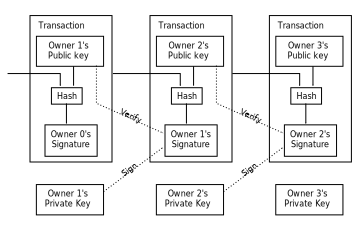
\includegraphics[width=\columnwidth]{img/Bitcoin_Transaction_Visual}
    \caption{A chain of digital signatures representing value transfer.
    (source \protect\cite{satoshi})}
    \label{fig:chain-spend}
\end{figure}

\begin{figure}[t!]
    \centering
    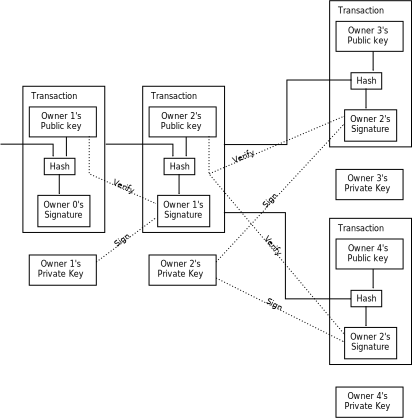
\includegraphics[width=\columnwidth]{img/Bitcoin_DoubleSpend_Visual}
    \caption{A chain of digital signatures representing value transfer with a double spend: Without some consensus system ``User 2'' is not prevented from sending the same value to both ``Owner 3'' and ``Owner 4''.
    (based on work from \protect\cite{satoshi})}
    \label{fig:chain-double-spend}
\end{figure}

The central authorities in this protocol also requires some degree of trust from the user that the authority is both benign and secure. For example, the central authorities could cooperate with, or more simply act as, a user attempting to achieve a double spend attack by showing different views to different users. Another reason that this currency was not adopted, was that a concrete implementation was never created and servers were never elected.

\section{The Bitcoin Protocol}
The Bitcoin protocol and client software~\textcite{satoshi} makes very few changes to the original b-money\cite{b-money} proposal. 

The Bitcoin protocol and client software provides a concrete implementation of an altered version of the original b-money proposal, with defined transaction syntax such as dynamic payment scripts and the concept of outputs that must be spent in their entirety.  The only significant novel deviation is that \textcite{satoshi} has substituted the ``synchronous and unjammable anonymous broadcast channel''~\cite{b-money} with a decentralized time stamp server that is used to ratify the order in which transactions occurred.  This allows for a dynamically changing set of transaction authorizing servers to achieve a consensus of valid transactions. Any user can, on receipt of a transaction, query the time stamp server and determine whether a transaction has been invalidated by a prior transaction. This key difference is likely the reason that Bitcoin took crypto-currencies from mathematical curiosity to a usable system for storage and transfer of value.

\subsection{Distributed Transaction Validation}
During the operation of the distributed time stamp server, the Bitcoin peer network, creates a chain of blocks of transactions, each referring to the previous by hash value. This is known as the Bitcoin block chain.  The transactions to be included in blocks in the chain are discovered when peers broadcast them into a peer discovery network that operates in a similar manner to a BitTorrent swarm\cite{swarm}.  Any user can contribute to this chain of blocks, but before another peer will relay it to others, it must meet a ``proof-of-work'' requirement: the double SHA-256 hash value of each block must not exceed a value determined by the current `difficulty'.  Because the SHA2 hashing function has been designed such that the value of an amount of data is unpredictable and evenly distributed in the range of the function, the only way for a participant to create data with a hash value below the difficulty limit is to repeatedly try different input data values\cite{btc-crypto}.  \textcite{satoshi} stated that ``The average work required is exponential in the number of zero bits required and can be verified by executing a single hash''. Transaction block data can be altered without changing the transaction semantics because the block format includes a `nonce' field for this purpose.

Because each block refers to the previous block, ``To modify a past block, an attacker would have to redo the proof-of-work of the block and all blocks after it''.  A peer in the Bitcoin network will accept a block if it has the highest total difficulty of any other block at that block height, shown in figure~\ref{ref:blockchain}, this allows the block chain to temporarily fork in the case that two blocks are created at the same time. The required difficulty of a valid block is re-calculated every 2016 blocks to ensure that block production takes the entire network an average of 10 minutes to solve.

\begin{figure}[t!]
    \centering
    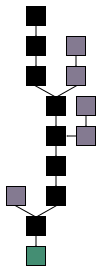
\includegraphics[height=\columnwidth]{img/Blockchain}
    \caption{A diagram showing invalid blocks (grey) being invalidated by a block chain with greater totaly difficulty (black). (based on work from theymos\protect\footnote{\url{http://theymos.com/}})}
    \label{fig:blockchain}
\end{figure}

As more blocks are created the more expensive it is for any group to alter the consensus reached by the peer network.  Because the proof-of-work system is computationally expensive, an incentive (other than the increased certainty of any transaction a user has previously received will remain valid) is included.  

While it is required that transactions included in a block have a total input value that exceeds the output value, one transaction, the `coinbase' transaction, can be included with no input and has a reward output.  The reward output is limited to the total difference between the input and output values of all other transactions in the block (as transaction fees), and a number related to the total number of blocks created by the network. Currently this reward is 25 bitcoins plus fees and is specified to halve every four years worth of blocks.  The intention is that the creator of the block assigns that reward to their own public key or address. This reward is `paid' for by the consensual deflation of every participants' held bitcoin. This process also serves to solve the distribution problem of digital currencies.

\subsection{The Bitcoin block chain is not strictly a consensus protocol}
\textcite{bitcoin-impossible} notes that, strictly, the Bitcoin proof-of-work block chain is not a consensus scheme. In distributed consensus protocols, consensus is arrived at when some sufficient number of members of the group agree.

This is impossible to achieve in a distributed system where this group is not known (agents are constantly joining and leaving the group) in a way that prevents Sybil attacks\cite{sybil} where an individual represents themselves as many agents, with the aim of overriding the group consensus.  By declaring the Bitcoin group consensus definition as ``all the computing power in existence'' consensus is only achieved once more than half of the compute power in existence is used in the proof-of-work system. Therefore the Bitcoin system is only Sybil \emph{resistant}. The Bitcoin systems is also not fully decentralized, a set of core developers, now the Bitcoin Foundation, have some control over the protocol; two major disruptions to the network have been solved using manual intervention from this group.  The first occurred on 15 August 2010 when an integer overflow was discovered in the Bitcoin protocol, this vulnerability ``allows remote attackers to bypass intended economic restrictions and create many bitcoins via a crafted Bitcoin transaction.''~\cite{CVE-2010-5139}. The second was when the network segmented two groups of clients with two differing consensus conclusions~\cite{CVE-2013-3220,glitch-report,major-glitch}.  Users of the network are still free to ignore the advice of this group by opting not to update or alter their clients in doing so permanently segregating themselves from the rest of the network.

\section{Anonymity}
As part of the Bitcoin protocol, all transactions must be broadcast publicly.  However, \textcite{satoshi} maintains that ``privacy can still be maintained by breaking the flow of information [...] by keeping public keys anonymous''.

Each Bitcoin address can be considered a pseudonym of the owner of it's associated private key, and because each person can own multiple Bitcoin addresses in a wallet there is a disconnect between users and addresses. \textcite{satoshi} asserts that because of this disconnect between users and addresses it is difficult to associate a particular transaction with a particular user.

\subsection{Taint Analysis}
\textcite{reid-anon}, consider the feasibility of maintaining this pseudo-anonymity in practise, by investigating the multiple input semantics of the Bitcoin transaction format. They argue that any key taking part in this process was in a single wallet, and thus owned by a single user. Therefore by combining the knowledge of how keys are grouped into wallets with knowledge from outside the protocol other inferences can be made, with the aim to determine the identity of the user behind the wallet, and thus any transactions made.  The proposed method for de-anonymizing a user occurs in two phases.  First, the publicly available ``transaction network'', as published in the block chain, is contracted to a ``user network'' by determining groups of addresses that appear to behave as part of a single wallet.  The second phase is to link that group with an identity using publicly available ``Off-Network Information'' linking users to any address in that group, e.g. by crawling the web for forum posts including both user-names and addresses.  \textcite{eval-priv} add to this a further heuristic of ``Shadow Addresses'' to associate newly created addresses with users.

\subsubsection{Multi-input Transactions}
In the Bitcoin transaction format, if a user cannot fulfil the value of a transaction by spending a single previous output, the client will combine multiple inputs, where the user has the ability to fulfil their spend conditions.  When combined, the Bitcoin client must fulfil the spend conditions of all of the inputs, usually the conditions result in the requirement to sign the transaction with all of the participating address's private keys.  ``It is therefore straightforward to conclude that if these (inputs) are (spendable) by different addresses, then the input addresses belong to the same user''\cite{eval-priv}, this is shown in figure~\ref{fig:multi-spend}.

\subsubsection{``Shadow'' or Change addresses}
Because each previous output must be redeemed in it's entirety, to support transactions of values smaller than the smallest output available to a wallet, the Bitcoin client automatically creates a new ``change address'' to send the remaining value to.  \cite{eval-priv} refers to this as a ``Shadow'' address.  The heuristic proposed, is that if money is sent to two or more addresses and only one has not been used before, that address is controlled by the user that created the transaction. A vulnerability in the Bitcoin client was that it never randomized the outputs of the addresses and so this change address always appeared in a known location in the serialized transaction\cite{cve-ordered-trans}. This is also shown in figure~\ref{fig:multi-spend}. To avoid this heuristic, a user must always ensure that they only send money to newly generated Bitcoin addresses.

\begin{figure}[t!]
    \centering
    \includegraphics[width=\columnwidth]{img/group_addresses}
     \caption{Two users send money to $k_{SR}$. Under the Multi-Input  heuristic $k_{a1}, k_{a2} and k_{a3}$ and $k_{b1}, k_{b2}$ are contracted into  some user $a$ and some user $b$. Under the change address heuristic  $k_{a4}$ and $k_{b3}$ are also contracted into user $a$ and user $b$  respectively. }
    \label{fig:multi-spend}
\end{figure}

\subsection{Taint Analysis Disruption}
\textcite{reid-anon} suggest repeatedly sending coins to new addresses, see Figure~\ref{fig:multi-new-addresses}. While this would gain anonymity under the reasoning of the paper, a new heuristic could be added to define that: for addresses that have not yet been spent, and therefore not linked with other addresses, those addresses should inherit the status of the addresses that sent to it.

\begin{figure}[t!]
    \centering
    \includegraphics[width=\columnwidth]{img/group_addresses}
      \caption{A user $a$ uses multiple new transactions to finally reach $k_a5$. }
    \label{fig:multi-new-addresses}
\end{figure}

\subsubsection{Fully Trusted Mixing}
\textcite{eval-priv} note that it is possible to use a mixing service to fully disrupt taint analysis.  A mixing service\footnote{\url{http://www.bitcoinlaundry.com/}} accepts Bitcoin transactions and automatically sends a new transaction otherwise unrelated with an equivalent output to a newly generated Bitcoin address.  These services often charge fees and require a significant amount of trust (bitcoin are totally in the control of the service before being returned).  The mixing service may also not have sufficient transaction traffic to be able to adequately hide the owner of bitcoin. Slight refinements on mixing services can be made by randomly adjusting the time that a transaction takes before being released or releasing multiple separate transactions into different newly generated addresses.

\subsubsection{ZeroCoin}
\textcite{zerocoin} propose a method of avoiding de-anonymization without a central trusted party, by defining new transaction types that take advantage of a zero knowledge proof (ZKP) that only proves knowledge of:

\begin{enumerate}
\item a Zerocoin in the block chain.
\item the actual serial number used to generate it.
\end{enumerate}

Formally, given all Zerocoins in the block chain ${C_1, C_2,\dots,C_N}$, prove knowledge of $C_i$ such that:

\begin{equation}
    (C_i = C_1) \vee (C_i=C_2) \vee \dots \vee (C_i=C_N)
\end{equation}

A ZKP for this statement is not efficient, as such, Zerocoin uses a one-way public accumulator with an efficient ZKP that accumulates ${C_1, C_2,\dots,C_N}$ to produce some $A$, such that it's possible to prove knowledge of a witness s.t. $C_i \in inputs(A)$~\cite{one-way-accumulators}.

The function used, equation~\ref{eqn:zkp}, that provides this mathematical property under the strong RSA assumption was proposed by \textcite{strong-rsa}.
%TODO: expand

A Zerocoin $C_{i}$ is created using serial number $S$ in the group $Z(N)$ using a Peterson commitment, equation~\ref{eqn:zq-create}, repeated until $C_i$ is a prime.

\begin{equation}\label{eqn:zq-create}
C_{i}=g^Sh^r, C_i \in \mathbb(P)
\end{equation}

An accumulator $A$ can be created from the asserted Zerocoins.  Adding to the accumulator is trivial, $A' = A*u^{C_i}$.

\begin{subequations}
    \begin{align}\label{eqn:zkp}
        N &= p \cdot q, u \in QR_{N}(u\neq1)\\
        A &= u^{C_1, C_2,\dots,C_N}\\
        w_i &=  u^{C_1, C_2,\cdots C_{i-1}, C_{i+1}, \dots ,C_N}
    \end{align}
\end{subequations}

Where $N$ is the product of two permanently private prime numbers - these primes are generated once, multiplied to derive $N$ then are permanently destroyed.

The zero knowledge proof, proves that $u^{C_i} \cdot w_i = A$. $w_i$ is now defined as the new accumulator. Unfortunately, this proof requires a 40KiB Double Discrete Logarithm proof, and the modification of all Bitcoin clients on the network which strictly is a new currency and no longer Bitcoin, but another incompatible block chain currency.

\subsubsection{In-Protocol Mixing}
In his forum post, ``I taint rich!'', Bitcoin developer Gregory (gmaxwell) Maxwell~\cite{taint-rich} describes a process to disrupt automated taint analysis.  Because the conditions of a set of previous outputs can be fulfilled partially, multiple users can cooperate to create a single transaction that causes their public keys to appear linked in a single wallet to taint analysis, without revealing their private keys to the group.  As such, the claim made by \textcite{satoshi}, and key assumption made by \textcite{reid-anon}, that some linking in multi-input transactions is unavoidable which necessarily reveals that inputs were owned by the same user, is false.

While participating in an example situation as described in Figure~\ref{fig:taint-rich}, it is clear how the addresses are truly linked in the user graph.  This is an artifact of the cooperation being performed on a public forum, the same address being used on the input and output as well as the fact that that address is the vanity address, ``1gmaxw''. The complexity of this process means it is not well used.

\begin{figure}[t!]
    \centering
    \includegraphics[width=\columnwidth]{img/taint_rich}
      \caption{$k_1$ and $k_2$ are owned by different users, yet grouped in the same transaction}
    \label{fig:taint-rich}
\end{figure}

A serious taint disrupting transaction must have the following three properties:  First, there should be no link between the inputs and the outputs other than the privately known ownership.  Secondly each output must utilise an address that has not been used previously. Thirdly, the transaction must not be traceable to a publicly identifiable network address and finally, the communication during cooperation must not be intercepted.  At this point, from the view of the block chain, the wallets used appear linked, under the multi-transaction heuristic and change address heuristic.

Below are two proposed methods of creating such transactions, both of which require a central server and a software client on the users' machines.

In the first method, the client initially generates a new address to receive bitcoin to, then multiple clients connect to a server operating a Tor\cite{tor} hidden service\footnote{This is used to prevent network addresses being known publicly} and each publishes outputs (the addresses) that they would like to assign value to.  All clients must now generate a new Tor identity and reconnect to the hidden service.  Finally, the server distributes a transaction with all of the outputs received to each client in turn to be signed.

The second involves a central server operating using a Tor hidden service which is used as a registration point for clients - each also operating a Tor hidden service.  Clients also operate a Tor hidden service and use the central server to register that particular Tor hidden service address and to discover other registered peers.  Each time a client wishes to mix coins, a random peer is chosen from the registry and is directly connected to via Tor, these clients now both agree on a multi-input transaction from both clients split equally between two new addresses. Assuming that the ownership of originating addresses was known publicly, the public knowledge ownership of the two new addresses is now split evenly between the two peers.  As each peer knows the true location of their own and, by a process of elimination, their peer's bitcoin this process must take place repeatedly between many different peers.

In both schemes the central service should be considered a weakness however, in both cases it is only trusted to operate as a routing service between peers the central system described in the second scheme could be replaced with a distributed peer discovery system similar to the Bitcoin peer discovery system.

In comparison to fully trusted mixing methods, the central server is only trusted as a means of registration rather than actually transacting money and maintaining the secrecy of the clients' identities.

One major disadvantage of these schemes is that it is possible for an attacker to cause a denial of service attack by refusing to sign a transaction that it requested thus rendering the entire transaction invalid.  While this is less of an issue in the second scheme, because multiple transactions are created with different peers thus a single defecting peer will not affect the entire swarm, this can be mitigated by making the protocol Sybil\cite{sybil} resistant by requiring a proof-of-work with each new address publication.

\section{Conclusion}
While it is clear that the de-anonymization techniques will no-longer be applicable once anonymization techniques including those discussed in this report become widely used by users of the Bitcoin system, it is not obvious that they will be applicable to existing network data. After all, any user that wished to remain anonymous who is also well versed in the protocol would have been able to avoid de-anonymization, even before the Bitcoin client\cite{bitcoin-qt} added support for multi-output transactions and before the dangers of address re-use were widely publicized because these techniques were already available when interacting with the network directly via command line tools.

\section{Future Work}
This report discusses a proposal for a novel anonymization system, an obvious avenue for further work would be to design, create and test a concrete implementation. Other avenues for further work would to be to investigate design changes and improvements to the existing Bitcoin system.  Further avenues of research could be to investigate enhancements to the Bitcoin protocol, for example using internet-wide multicast for transaction distribution.

% An example of a floating figure using the graphicx package.  Note that \label
    % must occur AFTER (or within) \caption.  For figures, \caption should occur
    % after the \includegraphics.  Note that IEEEtran v1.7 and later has special
    % internal code that is designed to preserve the operation of \label within
    % \caption even when the captionsoff option is in effect. However, because
    % of
% issues like this, it may be the safest practice to put all your \label just
    % after \caption rather than within \caption{}.
%
% Reminder: the "draftcls" or "draftclsnofoot", not "draft", class option should
    % be used if it is desired that the figures are to be displayed while in
    % draft mode.
%
%\begin{figure}[!t] \centering \includegraphics[width=2.5in]{myfigure} where an
    %.eps filename suffix will be assumed under latex, and a .pdf suffix will be
    %assumed for pdflatex; or what has been declared via
    %\DeclareGraphicsExtensions.  \caption{Simulation Results.} \label{fig_sim}
    %\end{figure}

% Note that IEEE typically puts floats only at the top, even when this results
    % in a large percentage of a column being occupied by floats.  However, the
    % Computer Society has been known to put floats at the bottom.


% An example of a double column floating figure using two subfigures.  (The
    % subfig.sty package must be loaded for this to work.) The subfigure \label
    % commands are set within each subfloat command, and the \label for the
    % overall figure must come after \caption.  \hfil is used as a separator to
    % get equal spacing.  Watch out that the combined width of all the
    % subfigures on a line
% do not exceed the text width or a line break will occur.
%
%\begin{figure*}[!t] \centering \subfloat[Case
    %I]{\includegraphics[width=2.5in]{box}% \label{fig_first_case}} \hfil
    %\subfloat[Case II]{\includegraphics[width=2.5in]{box}%
    %\label{fig_second_case}} \caption{Simulation results.} \label{fig_sim}
    %\end{figure*}
%
% Note that often IEEE papers with subfigures do not employ subfigure captions
    % (using the optional argument to \subfloat[]), but instead will
    % reference/describe all of them (a), (b), etc., within the main caption.


% An example of a floating table. Note that, for IEEE style tables, the \caption
    % command should come BEFORE the table. Table text will default to
    % \footnotesize as IEEE normally uses this smaller font for tables.  The
    % \label must come after \caption as always.
%
%\begin{table}[!t] % increase table row spacing, adjust to taste
    %\renewcommand{\arraystretch}{1.3} if using array.sty, it might be a good
    %idea to tweak the value of \extrarowheight as needed to properly center the
    %text within the cells \caption{An Example of a Table} \label{table_example}
    %\centering % Some packages, such as MDW tools, offer better commands for
%making tables % than the plain LaTeX2e tabular which is used here.
    %\begin{tabular}{|c||c|} \hline One & Two\\ \hline Three & Four\\ \hline
    %\end{tabular} \end{table}


% Note that IEEE does not put floats in the very first column - or typically
    % anywhere on the first page for that matter. Also, in-text middle ("here")
    % positioning is not used. Most IEEE journals use top floats exclusively.
    % However, Computer Society journals sometimes do use bottom floats - bear
    % this in mind when choosing appropriate optional arguments for the
    % figure/table
% environments.  Note that, LaTeX2e, unlike IEEE journals, places footnotes
    % above bottom floats. This can be corrected via the \fnbelowfloat command
    % of the stfloats package.

